% Author: Mark G.

\subsubsection{Description/additional circuitry}
% Describe how your electronic hardware brake plausibility system works (this is in addition to your ECU controlled brake plausibility software), provide tables with main operation parameters, and describe additional circuitry used to check or for an implausibility. Describe how the system reacts if an implausibility or error is detected.

BSPD is represented by a PCB with an on-board current transducer. It’s function is to monitor
power drawn from ACP and brake pedal pressure, and open SDC in case both signals are above
allowed threshold for more than 0,5 seconds. Also, the event of disconnection of SDC is latched,
thus it gets to reset only in case of the main power reset.



\begin{table}[H]
	\centering
	\caption{BSPD data}
	\begin{tabularx}{\textwidth}{|X|X|}
		\hline
		Brake sensor used: & Piezoresistive Pressure Transmitter PA-21Y / 100bar / 81691.1 \\[\TableSize]
		\hline
		Brake sensor physical response value: & Voltage, 4,5V \\[\TableSize]
		\hline
		Tractive system power sensor type & Current Transducer LEM HTFS 200-P \\[\TableSize]
		\hline
		Tractive system sensor physical response value: & Voltage of 85mV \\[\TableSize]
		\hline
		Tractive System power sensor current treshold (5kW/Nominal TS voltage): & 14A \\[\TableSize]
		\hline
		Supply voltages: & 5V \\[\TableSize]
		\hline
		Maximum supply currents: & 22mA \\[\TableSize]
		\hline
		Operating temperature: & -40..105$\circ$C\\[\TableSize]
		\hline
		Output used to control AIRs: & Open a MOSFET in SDC \\[\TableSize]
		\hline
	\end{tabularx}%
	\label{tab:addlabel}%
\end{table}%
\iffalse
\begin{figure}[H]
	\centering
	\includegraphics[width=\textwidth]{./img/bspd-position.jpg}
	\caption{BSPD flowchart.}
	\label{fig:BSPD-flowchart}
\end{figure}\fi

\subsubsection{Schematic}
%Describe the wiring, show schematics including the circuit board, show data regarding the cables and connectors used
The BSPD PCB is mounted on a HV wire in such manner, that the HV wire goes through the
current transducer. Current transducer provides analog voltage output of a value proportional to
actual current (resp. power) drawn from ACP. This voltage is amplified and is converted to twostate
logic levels voltage with the use of comparators. The value of “High” current signal logic level
is set to be at 5kW of power drawn from ACP (14A).

Brake state is measured in ECUP, converted with help of a comparator to two-state logic levels
voltage and is sent directly to BSPD via wiring.

Both logic signals are connected to NAND inputs. When both inputs are at “High” level, a
capacitor C1 starts to charge through resistance R16. When voltage on C1 is higher than 2,5V, a
comparator U1B sends signal to open SDC.

\begin{figure}[H]
	\centering
	\includegraphics[width=\textwidth]{./img/bspd-schematic.pdf}
	\caption{BSPD schematic sheet}
	\label{fig:BSPD-schematic}
\end{figure}

\subsubsection{Connection with shutdown circuit}
The connection to SDC is provided by an NPN transistor Q2 and a P-Channel MOSFET Q1, that
are connected to act as a “normally-closed” switch in SDC loop. Thus in case of a trip event Q1
stops conducting current between Drain and Source. See \ref{fig:BSPD-schematic}.

This state is latched by a latch-circuit, that consists of two NAND gates.

\iffalse
\begin{figure}[H]
	\centering
	\includegraphics[width=\textwidth]{./img/bspd-position.jpg}
	\caption{BSPD connection with SDC.}
	\label{fig:BSPD-conn}
\end{figure}\fi

\subsubsection{Position in car/mechanical fastening/mechanical connection}
%Provide CAD-renderings showing all relevant parts and discuss the mechanical connection of the sensors to the pedal assembly. Mark the parts in the rendering, if necessary.

BSPD is placed in Service Box, which connects high voltage harnesses from accumulator pack to motor controllers. The board containing BSPD circuit and current transducer is mounted to a wire.
\begin{figure}[H]
	\centering
	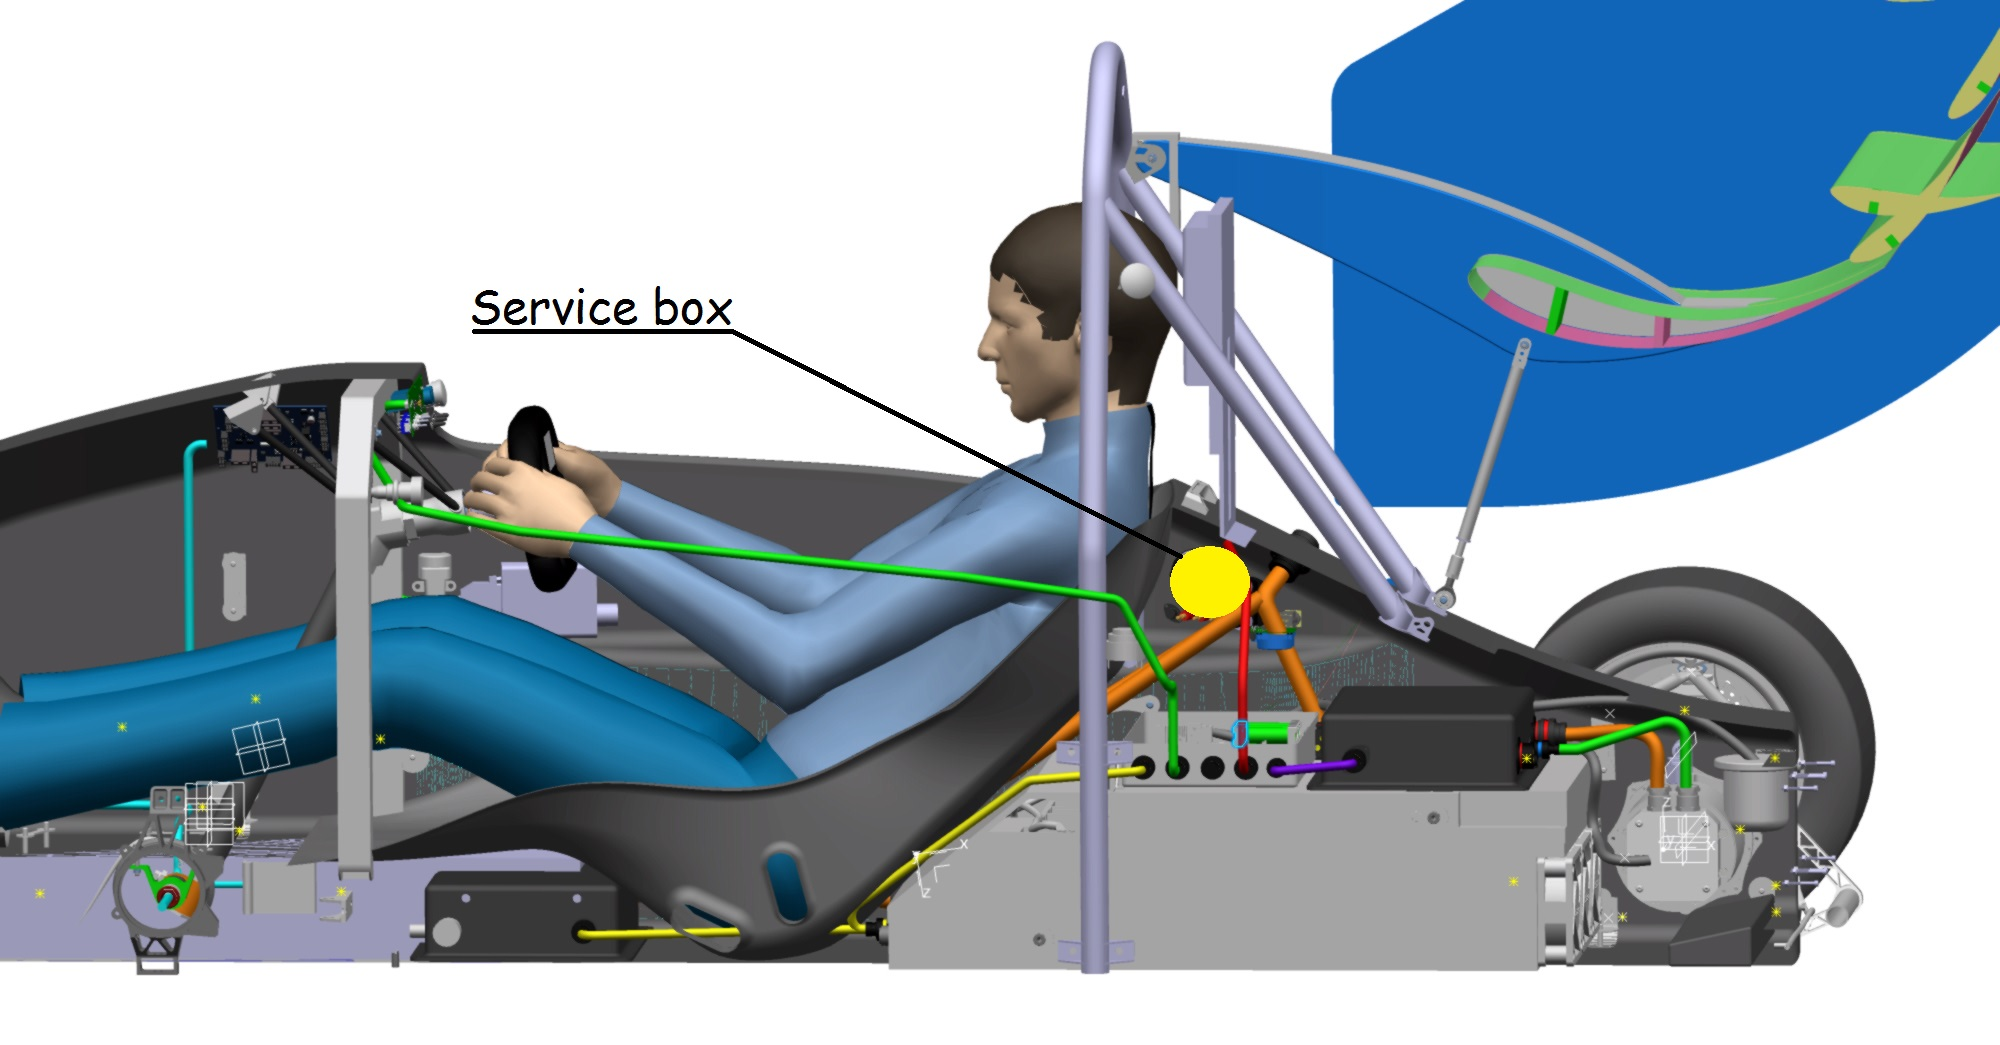
\includegraphics[width=\textwidth]{./img/ServiceBox-position.jpg}
	\caption{BSPD position}
	\label{fig:BSPD-position}
\end{figure}
